
%%% Local Variables:
%%% mode: latex
%%% TeX-master: "master"
%%% End:
\section{Two-Body Gravitational System}
Consider the following diagram
\begin{mycenter}



	\tikzset{every picture/.style={line width=0.75pt}} %set default line width to 0.75pt

	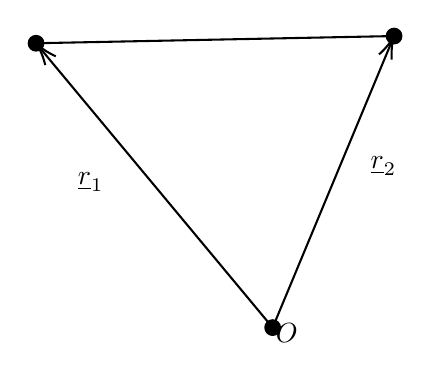
\begin{tikzpicture}[x=0.75pt,y=0.75pt,yscale=-1,xscale=1]
		%uncomment if require: \path (0,300); %set diagram left start at 0, and has height of 300

		%Shape: Circle [id:dp673844600958276]
		\draw  [fill={rgb, 255:red, 0; green, 0; blue, 0 }  ,fill opacity=1 ] (295.3,125.53) .. controls (295.3,123.58) and (296.88,122) .. (298.83,122) .. controls (300.78,122) and (302.37,123.58) .. (302.37,125.53) .. controls (302.37,127.48) and (300.78,129.07) .. (298.83,129.07) .. controls (296.88,129.07) and (295.3,127.48) .. (295.3,125.53) -- cycle ;
		%Straight Lines [id:da15576096830380182]
		\draw    (240.33,266) -- (298.06,127.38) ;
		\draw [shift={(298.83,125.53)}, rotate = 112.61] [color={rgb, 255:red, 0; green, 0; blue, 0 }  ][line width=0.75]    (10.93,-3.29) .. controls (6.95,-1.4) and (3.31,-0.3) .. (0,0) .. controls (3.31,0.3) and (6.95,1.4) .. (10.93,3.29)   ;
		%Shape: Circle [id:dp6113527558733022]
		\draw  [fill={rgb, 255:red, 0; green, 0; blue, 0 }  ,fill opacity=1 ] (236.8,266) .. controls (236.8,264.05) and (238.38,262.47) .. (240.33,262.47) .. controls (242.28,262.47) and (243.87,264.05) .. (243.87,266) .. controls (243.87,267.95) and (242.28,269.53) .. (240.33,269.53) .. controls (238.38,269.53) and (236.8,267.95) .. (236.8,266) -- cycle ;
		%Shape: Circle [id:dp5351046601993695]
		\draw  [fill={rgb, 255:red, 0; green, 0; blue, 0 }  ,fill opacity=1 ] (122.8,129) .. controls (122.8,127.05) and (124.38,125.47) .. (126.33,125.47) .. controls (128.28,125.47) and (129.87,127.05) .. (129.87,129) .. controls (129.87,130.95) and (128.28,132.53) .. (126.33,132.53) .. controls (124.38,132.53) and (122.8,130.95) .. (122.8,129) -- cycle ;
		%Straight Lines [id:da5024249129566511]
		\draw    (240.33,266) -- (127.61,130.54) ;
		\draw [shift={(126.33,129)}, rotate = 50.24] [color={rgb, 255:red, 0; green, 0; blue, 0 }  ][line width=0.75]    (10.93,-3.29) .. controls (6.95,-1.4) and (3.31,-0.3) .. (0,0) .. controls (3.31,0.3) and (6.95,1.4) .. (10.93,3.29)   ;
		%Straight Lines [id:da2152143947818559]
		\draw    (298.83,125.53) -- (126.33,129) ;

		% Text Node
		\draw (240.33,262.47) node [anchor=north west][inner sep=0.75pt]   [align=left] {$\displaystyle O$};
		% Text Node
		\draw (145,190) node [anchor=north west][inner sep=0.75pt]   [align=left] {$\displaystyle \underline{r}_{1}$};
		% Text Node
		\draw (286,182) node [anchor=north west][inner sep=0.75pt]   [align=left] {$\displaystyle \underline{r}_{2}$};


	\end{tikzpicture}

\end{mycenter}

We have 2 {\bf equations of motion} \eqref{eq: newtons-second-law}

\begin{align*}
	m\underline{\ddot{r_{1}}} = Gm_{1}m_{2}\frac{ \underline{r_{2}} - \underline{r_{1}}}{ \mid \underline{r_{2}} - \underline{r_{1}} \mid} \label{eq:
		two-body-grav-1} \tag{G1}
\end{align*}

\begin{align*}
	m\underline{\ddot{r_{1}}} = Gm_{1}m_{2}\frac{ \underline{r_{2}} - \underline{r_{1}}}{ \mid \underline{r_{2}} - \underline{r_{1}} \mid} \label{eq:
		two-body-grav-2} \tag{G2}
\end{align*}
Since the direction vectors are in opposite direction:

$$m_{1}\underline{\ddot{r_{1}}} + m_{2} \underline{\ddot{r_{2}}} = 0 \Rightarrow (m_{1} + m_{2}) = \underline{\ddot{R}} = 0$$

\clearpage
Consider the following diagram
\begin{mycenter}



	\tikzset{every picture/.style={line width=0.75pt}} %set default line width to 0.75pt

	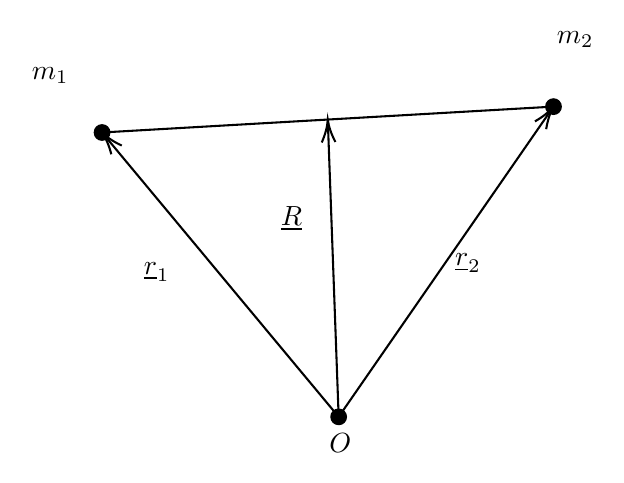
\begin{tikzpicture}[x=0.75pt,y=0.75pt,yscale=-1,xscale=1]
		%uncomment if require: \path (0,300); %set diagram left start at 0, and has height of 300

		%Shape: Circle [id:dp673844600958276]
		\draw  [fill={rgb, 255:red, 0; green, 0; blue, 0 }  ,fill opacity=1 ] (340.3,116.53) .. controls (340.3,114.58) and (341.88,113) .. (343.83,113) .. controls (345.78,113) and (347.37,114.58) .. (347.37,116.53) .. controls (347.37,118.48) and (345.78,120.07) .. (343.83,120.07) .. controls (341.88,120.07) and (340.3,118.48) .. (340.3,116.53) -- cycle ;
		%Straight Lines [id:da15576096830380182]
		\draw    (240.33,266) -- (342.69,118.18) ;
		\draw [shift={(343.83,116.53)}, rotate = 124.7] [color={rgb, 255:red, 0; green, 0; blue, 0 }  ][line width=0.75]    (10.93,-3.29) .. controls (6.95,-1.4) and (3.31,-0.3) .. (0,0) .. controls (3.31,0.3) and (6.95,1.4) .. (10.93,3.29)   ;
		%Shape: Circle [id:dp6113527558733022]
		\draw  [fill={rgb, 255:red, 0; green, 0; blue, 0 }  ,fill opacity=1 ] (236.8,266) .. controls (236.8,264.05) and (238.38,262.47) .. (240.33,262.47) .. controls (242.28,262.47) and (243.87,264.05) .. (243.87,266) .. controls (243.87,267.95) and (242.28,269.53) .. (240.33,269.53) .. controls (238.38,269.53) and (236.8,267.95) .. (236.8,266) -- cycle ;
		%Shape: Circle [id:dp5351046601993695]
		\draw  [fill={rgb, 255:red, 0; green, 0; blue, 0 }  ,fill opacity=1 ] (122.8,129) .. controls (122.8,127.05) and (124.38,125.47) .. (126.33,125.47) .. controls (128.28,125.47) and (129.87,127.05) .. (129.87,129) .. controls (129.87,130.95) and (128.28,132.53) .. (126.33,132.53) .. controls (124.38,132.53) and (122.8,130.95) .. (122.8,129) -- cycle ;
		%Straight Lines [id:da5024249129566511]
		\draw    (240.33,266) -- (127.61,130.54) ;
		\draw [shift={(126.33,129)}, rotate = 50.24] [color={rgb, 255:red, 0; green, 0; blue, 0 }  ][line width=0.75]    (10.93,-3.29) .. controls (6.95,-1.4) and (3.31,-0.3) .. (0,0) .. controls (3.31,0.3) and (6.95,1.4) .. (10.93,3.29)   ;
		%Straight Lines [id:da2152143947818559]
		\draw    (343.83,116.53) -- (126.33,129) ;
		%Straight Lines [id:da2561222159738197]
		\draw    (240.33,266) -- (235.16,124.77) ;
		\draw [shift={(235.08,122.77)}, rotate = 87.9] [color={rgb, 255:red, 0; green, 0; blue, 0 }  ][line width=0.75]    (10.93,-3.29) .. controls (6.95,-1.4) and (3.31,-0.3) .. (0,0) .. controls (3.31,0.3) and (6.95,1.4) .. (10.93,3.29)   ;

		% Text Node
		\draw (234.33,272.47) node [anchor=north west][inner sep=0.75pt]   [align=left] {$\displaystyle O$};
		% Text Node
		\draw (145,190) node [anchor=north west][inner sep=0.75pt]   [align=left] {$\displaystyle \underline{r}_{1}$};
		% Text Node
		\draw (295,186) node [anchor=north west][inner sep=0.75pt]   [align=left] {$\displaystyle \underline{r}_{2}$};
		% Text Node
		\draw (91,96) node [anchor=north west][inner sep=0.75pt]   [align=left] {$\displaystyle m_{1}$};
		% Text Node
		\draw (344,79) node [anchor=north west][inner sep=0.75pt]   [align=left] {$\displaystyle m_{2}$};
		% Text Node
		\draw (211,163) node [anchor=north west][inner sep=0.75pt]   [align=left] {$\displaystyle \underline{R}$};


	\end{tikzpicture}

\end{mycenter}

Put $\underline{r_{1}} = \underline{R} + \underline{s_{1}}$ and
$\underline{r_{1}} = \underline{R} + \underline{s_{2}}$

\begin{align*}
	m_{1} & \underline{\ddot{s_{1}}} = Gm_{1}m_{2}\frac{\underline{s_{2}} - \underline{s_{1}}}{\mid \underline{s_{2}} - \underline{s_{1}} \mid} \ \ \ \ \ \ \
	m_{2}\underline{\ddot{s_{2}}} = Gm_{2}m_{1}\frac{\underline{s_{1}} - \underline{s_{2}}}{\mid \underline{s_{1}} - \underline{s_{2}} \mid}                  \\ \\
	      & \text{and put
	} \underline{r} = \underline{r_{1}} - \underline{r_{2}} = {\underline{s_{1}} - \underline{s_{2}}}
\end{align*}

We get a {\bf second order differential equation}
$$\underline{\ddot{r}} = -G(m_{1}+m_{2})\frac{\underline{r}}{\mid \underline{r} \mid^{3}} = -\frac{GM\underline{r}}{\mid \underline{r} \mid}$$


\begin{note}
	$$\underline{s_{1}} = \frac{m_{2}\underline{r}}{m_{1}+m_{2}} \ \ \ \ \ \ \ \ \ \underline{s_{1}} = \frac{m_{2}\underline{r}}{m_{1}+m_{2}} $$
\end{note}

From an earlier result:

\begin{align*}
	E & = \frac{1}{2}m_{1}\mid \underline{r_{1}} \mid^{2} + \frac{1}{2}m_{2} \mid \underline{r_{2}} \mid^{2} - \frac{Gm_{1}m_{2}}{\mid \underline{r_{1}} - \underline{r_{2}} \mid}                                                                                        \\ \\
	  & = \frac{1}{2}m_{1} \mid \underline{R} + \underline{\dot{s_{1}}} \mid^{2} +  \frac{1}{2}m_{2} \mid \underline{R} + \underline{\dot{s_{2}}} \mid^{2} - \frac{Gm_{1}m_{2}}{\mid \underline{r_{1}} - \underline{r_{2}} \mid}                                          \\ \\
	  & = \frac{1}{2}m_{1} \left| \underline{\dot{R}} + \frac{m_{2}\underline{\dot{r}}}{m_{1} + m_{2}} \right|^{2}
	+ \frac{1}{2} m_{2}\left| \underline{\dot{R}} + \frac{m_{1}\underline{\dot{r}}}{m_{1} + m_{2}} \right|^{2}
	- \frac{Gm_{1}m_{2}}{\mid \underline{r_{1}} - \underline{r_{2}} \mid}                                                                                                                                                                                                 \\ \\
	  & =  \underbrace{\frac{1}{2}(m_{1} + m_{2})\left| \underline{\dot{R}} \right|^{2}}_{(1)} + \underbrace{\frac{1}{2}\frac{m_{1}m_{2}}{m_{1} + m_{2}}\left| \underline{r} \right|^{2}}_{(2)} - \frac{Gm_{1}m_{2}}{|\underline{r}|} \tag{$*G$} \label{eq:item-stuff-ke}
\end{align*}

\clearpage

In \eqref{eq:item-stuff-ke}, we have the following:
\begin{enumerate}
	\item $(1)$ is {\bf conserved} since center of mass acceleration is
	      constant and hence velocity is constant and therefore the {\bf Energy
			      associated with COM} is constant
	\item $(2)$ is nothing but Kinetic Energy + Potential Energy which is
		      {\bf constant} and hence {\bf conserved}.
\end{enumerate}
and therefore {\bf Energy in a 2 body gravitational system is conserved}

\subsection{Angular Momentum in a 2-body gravitational system}
By the definition of {\bf Angular Momentum} \eqref{eq: angular-momentum}
\begin{align*}
	\underline{J} & = m_{1}\underline{r_{1}} \times \underline{\dot{r_{2}}} + m_{2}\underline{r_{2}} \times \underline{\dot{r_{2}}}                                                             \\ \\
	              & = m_{1}(\underline{R} + \underline{s_{1}}) \times (\underline{R} + \underline{s_{!}}) + m_{2}(\underline{R} + \underline{s_{2}}) \times (\underline{R} + \underline{s_{2}}) \\ \\
	              & = (m_{1} + m_{2})(\underline{R} \times \underline{\dot{R}}) + m_{1}\underline{s_{1}} \times \underline{\dot{s_{2}}} + m_{2}\underline{s_{2}} \times \underline{\dot{s_{2}}} \\ \\
	              & = (m_{1} + m_{2})\underline{R} \times \underline{\dot{R}} + \frac{m_{1}m_{2}}{m_{1} +m_{2}}\underline{r} \times \underline{\dot{r}} \ \ \ \ \ \ \ \ \ \text{by
		substituting } \underline{s_{1}} \text{ and
	} \underline{s_{2}}                                                                                                                                                                         \\ \\
\end{align*}
and again these are both separately conserved as shown before in {\bf
		conservation of angular momentum},
since we the force is proportional to $\underline{r}$, i.e.
$$\underline{\ddot{r}} \propto \underline{r}$$
{\bf angular momentum is conserved}

\begin{remark}
	In the end, we do not need to care about the {\bf center of mass}
	\eqref{eq:com} motion since as it is a {\bf constant velocity motion and hence
			it is conserved} and has no contribution to angular momentum and energy of the system.
\end{remark}

\subsection{Reduced set of equations ignoring $\underline{R}$}
Ignoring $\underline{R}$, the system of equations gets reduced to

\begin{align*}
	\underline{\ddot{r}} & = -\frac{G(m_{1} + m_{2})}{| \underline{r}|^{3} }                                                            \\ \\
  \varepsilon          & = \frac{1}{2}\frac{m_{1}m_{2}}{m_{1} + m_{2}}|\underline{\dot{r}}|^{2} - \frac{Gm_{1}m_{2}}{|\underline{r}|} \\ \\
  \underline{L} &= \frac{m_{1}m_{2}}{m_{1} + m_{2}}\underline{r} \times \underline{\dot{r}}
\end{align*}

\clearpage
Here both $\underline{L}$ and $\underline{\varepsilon}$ are constants.

\begin{remark}
  Note that $\underline{L}$ is {\bf conserved} and {\bf perpendicular} to
  $\underline{r}$ and $\underline{\dot{r}}$ and therefore we can use polar co-ordinates.

\end{remark}

\begin{figure}[H]
\centering
   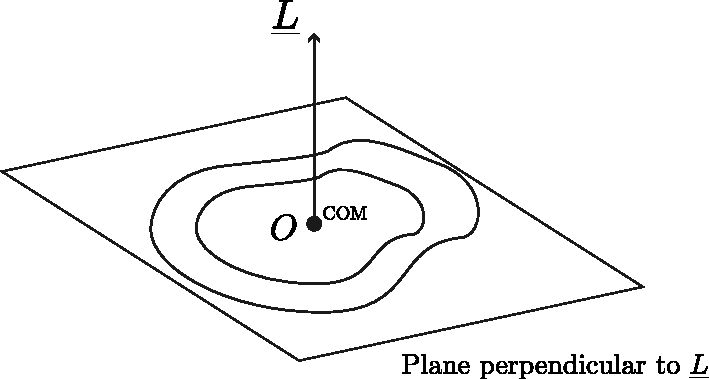
\includegraphics[scale=1.0]{2-body-grav.pdf}
   \label{fig:2-body-grav}
\end{figure}
